\documentclass[a4paper]{article}

\usepackage{cmap}
\usepackage[T2A]{fontenc}
\usepackage[utf8]{inputenc}
\usepackage[english,russian]{babel}
\usepackage{amsthm}
\usepackage{amssymb}
\usepackage{amsmath}
\usepackage{mathtools}
\usepackage{indentfirst}
\usepackage{fullpage}
\usepackage{titlesec}
\usepackage{multicol}
\usepackage{parskip}
\usepackage{graphicx}
\usepackage{tikz}
\usepackage{wrapfig}
\usepackage{breqn}

\newcommand{\open}{\underset{op}{\subset}}

\newtheoremstyle{definition}{3pt}{3pt}{\upshape}{}{\bfseries}{.}{.5em}{}
\theoremstyle{definition}
\newtheorem{definition}{Опр.}

\newtheoremstyle{statement}{3pt}{3pt}{\upshape}{}{\bfseries}{}{.5em}{}
\theoremstyle{statement}
\newtheorem{statement}{Утв.}
\newtheorem*{statement*}{Утв.}

\newtheoremstyle{lemma}{3pt}{3pt}{\upshape}{}{\bfseries}{}{.5em}{}
\theoremstyle{lemma}
\newtheorem{lemma}{Лемма}
\newtheorem*{lemma*}{Лемма}

\newtheoremstyle{note}{3pt}{3pt}{\upshape}{}{\bfseries}{:}{.5em}{}
\theoremstyle{note}
\newtheorem*{note}{Замечание}

\newtheorem{theorem}{Теорема}
\newtheorem*{theorem*}{Теорема}

\newtheoremstyle{example}{3pt}{3pt}{\upshape}{}{\bfseries}{:}{.5em}{}
\theoremstyle{example}
\newtheorem*{example}{Пример}

\title{Лекции по математическому анализу, 3 семестр}
\date{}
\author{Тимошенко Иван, 24123}


\begin{document}
    \maketitle
    \section{Модели комплексных чисел}

\par 
Введем стандартные понятия нужным образом:\\
$\mathbb{R}$ - множество точек на прямой. \\
$\mathbb{C}$ - расширение $\mathbb{R}$ с помощью одного из корней уравнения $z^2 = -1$: $\mathbb{C} = \mathbb{R} \cup  \{0\}$, с замыканием относительно сложения и умножения.

\begin{theorem}[Основная теорема алгебры]
    Множество комплексных чисел ($\mathbb{C}$) алгебраически замкнуто 
    (любой многочлен степени $n$, коэффициенты которого лежат в $\mathbb{C}$),
     имеет корни в $\mathbb{C}$ (с учетом кратности).
\end{theorem}

\begin{note}
    Теорема верна и в частном случае многочлена, определенного над $\mathbb{R}$.
\end{note}

\medskip
\subsection{Стандартная модель комплексных чисел}

Комплексное число $z$ представляется парой $(x, y) \in \mathbb{R}^2$ с операциями:
\begin{itemize}
    \item $"+": \quad (x_1, y_1) + (x_2, y_2) = (x_1+x_2, y_1 + y_2)$
    \item $"\cdot": (x_1, y_1) \cdot (x_2, y_2) = (x_1x_2-y_1y_2, x_2y_1+x_1y_2)$
\end{itemize}

\begin{note}
    Операции согласованы с операциями на $\mathbb{R}.$
\end{note}
\begin{note}
    $\mathbb{R} \subset \mathbb{C}, \quad \mathbb{R} = \{(x, 0) \quad x \in \mathbb{R}\}$
\end{note}
В станд. модели 
$\begin{cases}
    0 = (0, 0)\\
    1 = (1, 0)
\end{cases}$

\begin{definition}
    Мнимая единица определена как пара $(0, 1)$.
\end{definition}
\begin{note}
    Некорректно определять мнимую единицу как корень уравнения $z^2 = -1$, т.к. $-i$ так же является корнем.
    \[i^2 = (0, 1) \cdot (0,1) = (0\cdot0 - 1\cdot1, 0\cdot1 + 1\cdot0) = (-1, 0) = -1\]
    \[(-i^2) = (0, -1)\cdot(0, -1) = (-(-1)\cdot(-1), 0) = (-1, 0) = -1\]
\end{note}
\begin{note}
    Запись $\sqrt{-1}$ тоже некорректна.
\end{note}

\begin{statement}
    На $\mathbb{C}$ нельзя ввести линейный порядок.
    \begin{proof}
        Пусть $x \in \mathbb{C}$, и существует некий линейный порядок <.
        \[\forall x \neq 0
        \begin{cases}
            \text{либо} -\frac{x}{2} < \frac{x}{2} \text{ и } 0 = -\frac{x}{2} + \frac{x}{2} < \frac{x}{2} + \frac{x}{2} = x\\
            \text{либо} \frac{x}{2} < -\frac{x}{2} \text{ и } 0 > x
        \end{cases}
        \]
        Тогда $\forall x \neq 0$ либо $x > 0$, либо $-x > 0$. Т.е. $\forall x \neq 0 \quad x^2 > 0$.
        Но $-1 = i^2 < 0$ - противоречие.
    \end{proof}
\end{statement}

\bigskip

\subsection{Матричная модель}
Комплексное число $z = \begin{pmatrix}
    x & y\\
    -y & x
\end{pmatrix}$, где $x, y \in \mathbb{R}$.

\["+": 
    \begin{pmatrix}
        x_1 & y_1 \\
        -y_1 & x_1
    \end{pmatrix} 
    + 
    \begin{pmatrix}
        x_2 & y_2 \\
        -y_2 & x_2 \\
    \end{pmatrix}
    =
    \begin{pmatrix}
        x_1 + x_2 & y_1 + y_2 \\
        -y_1 - y_2 & x_1 + x_2
    \end{pmatrix}
\]
\["\cdot": 
    \begin{pmatrix}
        x_1 & y_1 \\
        -y_1 & x_1
    \end{pmatrix} 
    \cdot
    \begin{pmatrix}
        x_2 & y_2 \\
        -y_2 & x_2 \\
    \end{pmatrix}
    =
    \begin{pmatrix}
        x_1x_2 - y_1y_2 & x_1y_2 + x_2y_1 \\
        -x_1y_2 - x_2y_1 & x_1x_2 - y_1y_2
    \end{pmatrix}
\]

В матричной модели ноль (нейтральный элемент по сложению) представлен матрицей
$0 =\begin{pmatrix}
    0 & 0 \\
    0 & 0
\end{pmatrix}$, единица (нейтральный по умножению)
$1 = \begin{pmatrix}
    1 & 0 \\
    0 & 1
\end{pmatrix}$, мнимая единица  
$i = \begin{pmatrix}
    0 & 1 \\
    -1 & 0
\end{pmatrix}$.

В стандартной модели произвольное комплексное число $z = (x, y)$ 
имеет стандартную запись \\$z = x + iy$, где $\begin{cases}
    x - \text{вещественная часть}\\
    y = \text{мнимая часть}
\end{cases}$

Действия с комплексными числами:
\begin{enumerate}
    \item Сравнение (проверка равенства):
        \[a + ib = c + id \iff a = c \text{ и } b = d\].
    \item Сложение:
        \[(a+ib) + (c+id) = (a+c) + i(b+d)\]
    \item Умножение:
        \[(a+ib)\cdot(c+id) = (ac - bd) + i (ad + bc)\]
    \item Деление:
        \[\frac{a+ib}{c+id} = \frac{(a+ib)\cdot(c-id)}{c^2+d^2} = \frac{(ac - bd) + i(bc - ad)}{c^2 + d^2}\]
\end{enumerate}


\subsection{Геометрическая модель}

Комплексное число представлено точкой с координатами $(x, y)$ на плоскости.\\
Операции:
\begin{itemize}
    \item $"+"$: действует как сложение векторов (покоординатно).
    \item $"\cdot": z_3 = z_1z_2 \iff \begin{cases}
        |z_3| = |z_1|\cdot|z_2| \\
        arg(z_3) = arg(z_1) + arg(z_2)
    \end{cases}$
    \\ где $|z| = \sqrt{x^2 + y^2}, \quad arg(z)$ задает угол между $\vec{z}$ и Ox 
    (определяется с точностью до периода).
\end{itemize}

\textbf{Аргумент комплексного числа} $Arg(z)$ - угол $\varphi$ c точностью до периода $2\pi$.
\textbf{Главное значение аргумента} $arg(z)$ - $\varphi$  в промежутке $[0; 2\pi]$.

\textbf{Комплексно сопряженное к} $z = x+iy$ это $\overline{z} = x - iy$.
\[|z| = |\overline{z}|, \quad arg(z) = -arg(\overline{z}), \quad 
Re(z) = Re(\overline{z}), \quad Im(z) = -Im(\overline{z})\] 
\[\overline{z} \cdot z = (x+iy)\cdot(x-iy) = x^2 + y^2 = |z|^2\] 

\textbf{Законы де Моргана:}
\begin{itemize}
    \item $\overline{(\overline{z})} = z$
    \item $\overline{z_1 + z_2} = \overline{z_1} + \overline{z_2}$
    \item $\overline{z_1z_2} = \overline{z_1} \cdot \overline{z_2}$
\end{itemize}

\textbf{Неравенство треугольника:}
\[\begin{cases}
    |z_1 + z_2| \leq |z_1| + |z_2|\\
    |z_1 - z_2| \geq \lvert \lvert z_1\rvert - \lvert z_2\rvert \rvert
\end{cases} \implies \lvert \lvert z_1 \rvert - \lvert z_2 \rvert \rvert \leq 
\lvert z_1 + z_2 \rvert \leq \lvert z_1 \rvert + \lvert z_2 \rvert \]

\subsection{Стереографическая проекция}
На комплексную плоскость положили сферу $S$ радиуса $\frac{1}{2}$. Северный полюс сферы - вершина $N(0; 0; 1)$.
Комплексному числу $c$, лежащему в плоскости комплексных чисел и имеющему координаты $(x, y, 0)$ ставится в соответствие точка, которая является точкой пересечения прямой $Nc$ со сферой $S$. 
Зададим систему координат $O\xi \eta \zeta$ аналогично $Oxyz$, 
но $O$ имеет координаты $(0, 0, \frac{1}{2})$.\\
Уравнение сферы S:
\begin{equation} 
    \label{RimanSphereEq}
    \xi^2 + \eta^2 + (\xi - \frac{1}{2})^2 = (\frac{1}{2})^2
\end{equation}
Уравнение прямой $Nc$ по двум точкам:
\begin{equation}
    \label{NcEq}
    \frac{\xi}{x} = \frac{\eta}{y}=\frac{\zeta-1}{-1} 
    \iff
    \xi^2 + \eta^2 + \zeta^2 - \zeta = 0
\end{equation}

Получаем набор \textbf{обратных формул стереографической проекции:}
$x = \frac{\xi}{1 - \zeta}, y = \frac{\eta}{1-\zeta}, z = \frac{\xi + i\eta}{\zeta - 1}$.
Отсюда найдем
\begin{equation}
    \label{zsphere}
    \left| z \right|^2 = z \cdot \overline{z} = \frac{\xi^2 + \eta^2}{(1-\zeta)^2}
    \underset{\text{из } \ref{NcEq}}{=} \frac{\zeta}{1-\zeta} 
    \implies \zeta = \frac{\left| z \right|^2}{1 + \left| z\right|^2}
\end{equation}
Подставим \ref{zsphere} в уравнение \ref{RimanSphereEq} и получим прямые формулы стереографической проекции:
\begin{equation}
    \xi = \frac{x}{1 + \left|z\right|^2}, \quad
    \eta = \frac{y}{1 + \left|z\right|^2}, \quad
    \zeta = \frac{\left|z\right|^2}{1 + \left|z\right|^2}
\end{equation}

Из геометр. постреония стереографическая проекция взаимно однозначно 
отображает комплексную плокость на сферу $S \setminus \{N\}$.
Дополним стер. проекцию по непрерывности:
\begin{equation}
    P: \overline{\mathbb{C}} \overset{\text{на}}{\to}S \quad
    \text{где } \overline{\mathbb{C}} = \mathbb{C} \cup \{\infty\}, \text{а $S$ называют сферой Римана.}
\end{equation}

\begin{definition}
    Обобщенная окрестность на комплексной плоскости - это любая окружность (или прямая, рассмотренная как окружность бесконечного радиуса).
\end{definition}

Свойства стереографической проекции:
\begin{enumerate}
    \item Для любой обобщенной окружности $l \subset \overline{\mathbb{C}}$ ее образ $P(l) \subset S^2$ - это окружность.
    \begin{proof}
        Пусть $l$ - некая обобщ. окрестность на $\overline{\mathbb{C}}$, тогда ее уравнение:
        \[l: A(x^2+y^2) + Bx + Cy + D = 0 \text{ - окружность при $A \neq 0$, прямая при $A = 0$}\]
        Подставим в него обратные формулы стереогр. проекции:
        \begin{equation}
            A\frac{\zeta}{1 - \zeta} + B\frac{\xi}{1 - \zeta} + C\frac{\eta}{1 - \zeta} + D = 0
        \end{equation}
        Поделим на $1 - \zeta$ и получим:
        \begin{equation}
            \label{FlatEq}
            \text{П: }B\xi + C\eta + (A-D)\zeta + D = 0
        \end{equation}
        Но это уравнение некоторой плоскости П в $\mathbb{R}^3$, кроме того, $P(l) \subset S^2$,
        значит для $l$ выполнено уравнение сферы Римана $\xi^2 + \eta^2 + \zeta^2 - \zeta = 0$.
        Тогда $P(l) = S^2 \cap \text{П}$ - пересечение сферы с плоскосью окружность.
    \end{proof}

    \item $\forall$ окружности $L \subset S^2 \ P^{-1}(L)$ является обобщенной окружностью на $\overline{\mathbb{C}}$.
    \begin{proof}
        Плоскость $\Pi \subset \mathbb{R}^3$ такая, что $\Pi \cap S^2 = L$,
        а значит ее уравнение имеет \\ вид (\ref{FlatEq}). Разделим (\ref{FlatEq}) на $1-\zeta$, получим обобщенное уравнение прямой,
        подставим туда прямые формулы проекции и получим уравнение вида $A(x^2+y^2)+Bx +Cy + D = 0$, а это - уравнение обобщенной окружности в $\overline{\mathbb{C}}$.
    \end{proof}

    \item Стереографическая проекция сохраняет углы. То есть $\forall l_1, l_2 \in \overline{\mathbb{C}} \text{ таких, что } l_1 \cap l_2 \neq \empty$
    и $\alpha$ - угол между ними, верно, что угол между $P(l_1)$ и $P(l_2)$ тоже равен $\alpha$ (угол между окружностями это угол
    между касательными в точке пересечения).
\end{enumerate}

\begin{definition}
    Кривая - это функция (или ее образ) $g: [a, b] \to \mathbb{R}^2$. Параметром кривой $g$ называют $t \in [a, b]$. 
    \[\overrightarrow{v} = \frac{\frac{\partial \overrightarrow{g}}{\partial t}}{\left| \frac{\partial g}{\partial t}\right|} = \left( \frac{\frac{\partial x}{\partial t}}{\left| \frac{\partial g}{\partial t}\right|}, \ \frac{\frac{\partial y}{\partial t}}{\left| \frac{\partial g}{\partial t}\right|} \right) \quad \overrightarrow{n} = \frac{\frac{\partial^2 g}{\partial t^2}}{\left| \frac{\partial^2 g}{\partial t^2} \right|}\]
    Натуральный параметр на кривой $g$ это $l \subset [0, L]$ ($L$ - длина $g$), такой, что $\forall l$ выполнено $\frac{\partial g}{\partial l} = 1$.
    Набор $\{v, n\}$ называется базис Френе, для него выполена теорема Френе. 
    Уравнения Френе:
    \[
    \frac{d}{dl} \begin{pmatrix} v \\ n \end{pmatrix} = 
    \begin{pmatrix}
        0 & k(l) \\
        -k(l) & 0
    \end{pmatrix}
    \begin{pmatrix} v \\ n \end{pmatrix}, \quad k(l) \text{ называется кривизной } g \subset \mathbb{R}^2
    \]
\end{definition}

\subsection{Виды записи}
Стандартная запись $z = x + iy$. \\
Пусть $r = \left| z \right|, \ \varphi = arg(z)$.
\begin{definition}
    Тригонометрическая запись комплексного числа:
    \[\begin{cases}
        Re(z) = x = r\cdot \cos(\varphi) \\ 
        Im(z) = y = r\cdot \sin(\varphi)
    \end{cases} \implies z = x +iy = r(\cos(\varphi) + i\sin(\varphi))\]
\end{definition}
    
\begin{definition}
    Формула Эйлера:
    \[e^{i\varphi} = \cos(\varphi) + i\sin(\varphi) \implies z = re^{i\varphi}\]
    Тогда для натурального $n$:
    \[z^n = r^n e^{in\varphi} = r^n (\cos(n\varphi) + i\sin(n\varphi))\]
    Пусть $z \neq 0 \implies r = \left| z \right| > 0$. тогда $z^{\frac{1}{n}} = r^{\frac{1}{n}}\cdot e^{\frac{i(\varphi + 2\pi k)}{n}}$, где $k = 0 \hdots n-1$.
    Отсюда же получается формула Муавра для корней степени $n$ из $z \neq 0$:
    \[z^{\frac{1}{n}} = r^{\frac{1}{n}}(\cos(\frac{\varphi + 2\pi k}{n})+ i\sin(\frac{\varphi + 2\pi k}{n}))\]
\end{definition}

\begin{note}
    $\exists n$ различных корней степени $n$ из комплексного числа $z \neq 0$.
    \[z_0, z_1, \hdots z_{n-1} \in \text{ окружности радиуса } r^{\frac{1}{n}} \text{ c центром в } (0,0)\]
\end{note}

    \begin{definition}
    Функция дифференциируема в точке, если 
    \begin{itemize}
        \item $f:U \to \mathbb{R}^k$ и $p \in Int(U)$
        \item $f(x) = f(p) + df(p)\langle x-p \rangle + \alpha(x),$ где $\alpha(x) = o(x-p).$
    \end{itemize}
\end{definition}
Если $k = 1$, то лин. отображение $df(p):\mathbb{R}^n \to \mathbb{R}$
можно задатьа как $df(p)\langle v \rangle = \langle \nabla f(p);  v \rangle$
 - скалярное произведение градиента функции на вектор, причем 
 $\nabla f(p) = \left(\frac{\partial f}{\partial x_1}(p), \dots, \frac{\partial f}{\partial x_n}(p)\right)$ - вектор частных производных в точке $p$.

\begin{statement}
    Градиент функции задает направление, при движении в котором функция растет быстрее всего.
    \begin{proof}
        Рассмотрим функцию $f$ в точке $p$, вектор $v$ единичной длины будет задавать произвольное направление.
        \begin{equation*}\frac{f(p+tv) - f(p)}{t} \underset{t \to 0}{\to}
            \frac{\partial f}{\partial v} = df(p)\langle v \rangle = \langle \nabla f(p); v \rangle 
            = |\nabla f(p)| \cdot |v| \cdot cos(\varphi), \text{где $\varphi $ - угол между $\nabla f$ и $v$.}
        \end{equation*}
        Поскольку $|\nabla f(p) = const, |v| = 1$, то для максимизации надо выбрать такое $\varphi$, 
        чтобы $cos(varphi)$ был максимален, т.е. вектора $v$ и $\nabla f$ параллельны и $\nabla f$ задает наибольшую скорость роста.
    \end{proof}
\end{statement}

\begin{statement}
    $\nabla f(p)$ ортогонален поверхности уровня $\Omega = \{x | f(x) = c\}$.
    \begin{proof}
        Пусть $f(p) = c \ (p \in \Omega)$. Пусть $x_n \in \Omega$, покажем, что $cos(\nabla f(p), \overrightarrow{x_n-p}) \underset{n \to \infty}{\to} 0:$
        \begin{eqnarray*}
            f(x_n) = f(p) = c \implies 0 = f(x_n) - f(p) = df(p)\langle x_n-p \rangle + o(x_n - p) = 
            \langle \nabla f(p); x_n - p \rangle + o(x_n - p).
        \end{eqnarray*}
        Значит $0 \underset{n \to \infty}{=} \langle \nabla f(p); \frac{x_n - p}{|x_n - p|} \rangle + o(1)$, т.е.
        $\langle \nabla f(p); \frac{x_n - p}{|x_n - p|} \rangle \to 0 $. Тогда:
        \begin{equation*}
            \langle \nabla f(p); \frac{x_n - p}{|x_n - p|} \rangle = |\nabla f(p)|\cdot \left|\frac{x_n-p}{|x_n-p|}\right|\cdot cos(\alpha) \to 0, 
            \ \text{т.е.} \alpha \underset{n \to \infty}{\to} \frac{\pi}{2}. 
        \end{equation*}
        
    \end{proof}
\end{statement}

\begin{definition}
    Функция $f:\mathbb{R}^n \to \mathbb{R}^n$ называется векторным полем.
\end{definition}
\begin{definition}
    Потенциалом векторного поля $F$ (если он есть) называется \textbf{скалярная} функция $U:W \to \mathbb{R}$, 
    такая, что $\nabla U = F$. Если потенциал существует, то F называется потенциальным полем.

\end{definition}

\begin{theorem*}
    Пусть $f:U \subset \mathbb{R}^n \to \mathbb{R}^k, \ g:V \subset \mathbb{R}^k \to \mathbb{R}^m, \ f \in C^1(p), \ g \in C^1(q), \ q = f(p)$.\\
    Тогда $g \circ f \in C^1(p), \, dg \circ f = dg(f(p)) \cdot df(p).$ В матрицах Якоби: $D_{g \circ f}(p) = D_g(f(p)) \cdot D_f(p).$
\end{theorem*}

\begin{example}
    \begin{equation*}
        \begin{cases}
            f(x, y, z) = (xy, xz): \mathbb{R}^3 \to \mathbb{R}^2\\
            g(a, b) = \cosh(ab): \mathbb{R}^2 \to \mathbb{R}
        \end{cases} \quad
        f =
        \begin{cases}
            f_1(x, y, z) = xy\\
            f_2(x, y, z) = xz.
        \end{cases}
    \end{equation*}

    \begin{equation*}
        h = g(f(x, y, z)) = \cosh(xy \cdot xz): \mbox{R}^3 \to \mathbb{R}, \quad (x, y, z) \in \mathbb{R}^3 \overset{f}{\to} \mathbb{R}^3 \overset{g}{\to} \mathbb{R}
    \end{equation*}
    \begin{equation*}
        \frac{\partial h}{\partial x} = \sinh(x^2yz)\cdot 2xyz \quad
        \frac{\partial h}{\partial y} = \sinh(x^2yz)\cdot x^2z \quad
        \frac{\partial h}{\partial z} = \sinh(x^2yz) \cdot x^2y
    \end{equation*}

    \[D_f(x, y, z) = \begin{pmatrix}
        \frac{\partial f_1}{\partial x} & \frac{\partial f_1}{\partial y} &  \frac{\partial f_1}{\partial z} \\
        \frac{\partial f_2}{\partial x} & \frac{\partial f_2}{\partial y} &  \frac{\partial f_2}{\partial z}  
    \end{pmatrix} =
    \begin{pmatrix}
        y & x & 0 \\
        z & 0 & x
    \end{pmatrix}
    \]

    \[D_f = \begin{pmatrix}
        \sinh(ab)\cdot a & \sinh(ab) \cdot b
    \end{pmatrix}\]

    \[D_g \cdot D_f = \begin{pmatrix}
        \sinh(x^2yz)\cdot xz & \sinh(x^2yz)\cdot xy
    \end{pmatrix} \cdot \begin{pmatrix}
        y & x & 0 \\
        z & 0 & x
    \end{pmatrix}
    \]
    Досчитывать я это не буду, поверим Сторожуку на слово.
\end{example}

\textbf{Правило дифференциирования обратного отображения:}
Если невырождено и $\exists$ обратное отображение $g:V \to U$, непрерывное в точке $q = f(p)$, тогда:
\[g \in D(q) \text{ и } dg(q) = (df(p))^{-1}\]


\subsection{Многократная дифференциируемость}

\begin{definition}
    $f: U \subset \mathbb{R}^n \to \mathbb{R}^m \ k$ раз дифференциируема в точке $p$ ($f \in D^k(p)$), если:
    \begin{enumerate}
        \item $f$ дифференциируема во всех точках некоторой окрестности точки $p$;
        \item Все частные производные $\frac{\partial f}{\partial x_1}, \dots, \frac{\partial f}{\partial x_n}$ дифференциируемы $k-1$ раз в точке $p$.
    \end{enumerate}  
\end{definition}

\begin{example}
    \[f \in D^2(p) \implies f \in D(x) \text{ и } \frac{\partial f}{\partial x}, \frac{\partial f}{\partial y} \in D(p)  \]
\end{example}

\begin{statement*}
    Если $\begin{cases}
        f \in D^k(p): \mathbb{R}^n \to \mathbb{R}^k\\
        g \in D^k(p): \mathbb{R}^n \to \mathbb{R}^k
    \end{cases}$ тогда $h(x) = f(x) \cdot g(x) \in D^k(p)$

    \begin{proof}
        \begin{equation*}
            \frac{\partial h}{\partial x_i}(x) = \frac{\partial f}{\partial x_i}(x)\cdot g(x) +
            f(x) \cdot \frac{\partial g}{\partial x_i}
        \end{equation*}
        Так как $\frac{\partial f}{\partial x_i}(x) \in D^{k-1}(p), \ g(x) \in D^k(p), \ f(x) \in D^k(p), \ \frac{\partial g}{\partial x_i} \in D^{k-1}(p)$,
        то $\frac{\partial h}{\partial x_i} \in D^{k-1}(p)$.
    \end{proof}
\end{statement*}


\begin{theorem}[о вторых производных]
    Пусть $f:U \subset \mathbb{R}^n \to \mathbb{R}, \ f \in D^2(p)$. Тогда $\frac{\partial^2 f}{\partial x \partial y} = \frac{\partial^2 g}{\partial y \partial x}$.
    \begin{proof}
        Можно считать, что $n = 2$, так как при заданной функции $f(x_1, x_2, \dots)$ можно в качестве $f$ рассмотреть 
        сужение $f$ на плоскость $Ox_1x_2$, т.к. при дифференциировании по $x_1$ или $x_2$ остальные переменные не изменются.

        \[f = f(x, y) \in D^2(p), \quad p = (x_0, y_0, \dots)\]
        Считаем, что $p = 0$ и что $\frac{\partial f}{\partial x}(0) = 0, \ \frac{\partial f}{\partial y}(0) = 0$.
        Чтобы показать почему так можно считать введем $f_1$:
        \[f_1(x, y) := f(x,y) - f'_x(0, 0)\cdot x - f'_y(0,0)\cdot y\]
        \[\frac{\partial f_1}{\partial x}(0, 0) = \frac{\partial f}{\partial x}(0, 0) - f'_x(0,0)\]
        \[\frac{\partial f_1}{\partial y}(0,0) = \frac{\partial f}{\partial y}(0,0) - f'_y(0,0)\]
        
        Дальше считаем, что $f = f_1$ и $f(0,0) = 0$. 
        \begin{equation*}
            \frac{\partial f}{\partial x }(x, y) =f(0,0) + a_{11}\cdot x + a_{12}\cdot y + \alpha_1(x, y), \ \text{где }
            \alpha_1(x, y) = o(x, y), \ (a_{11}, a_{12}) = df(0,0)\langle x, y \rangle
        \end{equation*}
        По условию $\frac{\partial f}{\partial x}, \frac{\partial f}{\partial y} \in D(0)$, поэтому 
        $a_{11} = f_{xx}(0), \ a_{12} = f_{xy}(0)$.
        \[\frac{\partial f}{\partial y}(x, y) = f(0,0) + a_{21}\cdot x + a_{22}\cdot y + \alpha_2(x, y), \ 
        a_{21} = f_{yx}(0), \ a_{22} = f_{yy}(0)\]

        \newpage
        \begin{minipage}[t]{0.45\textwidth}        
            \begin{tikzpicture}[remember picture, overlay]
                \node[anchor=north west, yshift=5pt, xshift=10pt] at (current page.north west) {
                    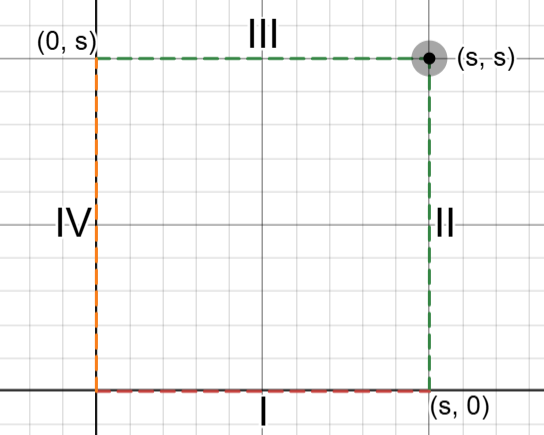
\includegraphics{График_для_теоремы_Шварца.png}
                };
            \end{tikzpicture}
        \end{minipage}
        \begin{minipage}[t]{0.5\textwidth}
            Рассмотрим точку $(s,s)$ вблизи нуля. Для нее 
            $f(s,s) - f(0,0) = (f(s,s) - f(s, 0)) + (f(s,0) - f(0,0)) = (II) + (I)$. \newline
            И в то же время $f(s, s) =  (\text{IV}) + (\text{III})$
        \end{minipage}
        \\[100pt]
        \[\text{II} = f(s,s) - f(s,0) = \int_{y=0}^{s}\frac{\partial f}{\partial y}(s,t)dt
        = \int_{t=0}^{s}a_{21}s + a_{22}t + \alpha_2(s,t)dt = a_{21}s^2 + \frac{a_{22}s^2}{2} + \varepsilon_1(s),\]
        причем $\varepsilon_1(s) = \int_{t=0}^{s}\alpha_2(s,t)dt$. Аналогично для I:
        \[\text{I} = f(s,0) - f(0,0) = \int_{t=0}^{s}\frac{\partial f}{\partial x}(t,0)dt = \int_{t=0}^{s}a_{11}t+a_{12}\cdot0 + \alpha_1(t)dt = 
        \frac{a_{11}}{2}s^2 + \varepsilon_2(s), \ \varepsilon_2(s) = \int_{t=0}^{s}\alpha_1(t,0)dt\]
        
        Итого: $f(s,s) - f(0,0) = \text{I} + \text{II} = s^2 \left( a_{21} + \frac{a_{11}}{2} + \frac{a_{22}}{2}+ \frac{\varepsilon_1(s) + \varepsilon_2(s)}{s^2}\right)$, что на самом деле равно $\text{III} + \text{IV} = 
        \\ = s^2\left(a_{12} + \frac{a_{11}}{2} + \frac{a_{22}}{2} + \frac{\varepsilon_3(s) + \varepsilon_4(s)}{s^2}\right)$
        
    
    \end{proof}
\end{theorem}
    \textbf{Правило дифференциирования монома:\\}
\bigskip
Пусть $f(x)  = x_1^{i_1} \cdot x_2^{i_2} \cdot \dots \cdot x_m^{i_m}, \ x = (x_1, \dots, x_m)$. Тогда 
\[\frac{\partial^{i_1+i_2+ \dots + i_m} f}{\partial x_1^{i_1} \dots \partial x_m^{i_m}}(0) = i_1! \cdot \hdots \cdot i_m!\]
Любая другая производная любого порядка в точке $0$ равна $0$.

\subsection{Мульти-индексы}
Придумаем $\mu = (i_1, \hdots, i_m)$ - численный вектор, в котором $\forall j = \overline{1 \hdots m} \ i_j \geq 0$ и назовем его \textbf{мультииндексом}.
\par
Для мультииндексов определены операции:
\[\mu! := i_1! \cdot \hdots \cdot  i_m! \qquad \left| \mu \right| = \sum_{j = 1}^{m} i_j \text{ - порядок мультииндекса}\]
\[x \in \mathbb{R}^m, x = (x_1, \hdots, x_m), \quad x^{\mu} = x_1^{i_1} \cdot \hdots \cdot x_m^{i_m}\]
\[C^{\mu}_k = \frac{k!}{\mu!} = \frac{k!}{i_1!\cdot \hdots \cdot i_m!} \text{, где } k = \left|\mu\right|\]

\bigskip

Зададим контекст:
\[f:\mathbb{R}^m \to E, \ f \in D^k(p), \ \mu = (i_1, \hdots, i_m)\]
Тогда:
\[\frac{\partial^{\mu}f}{\partial x^{\mu}} = D^{\mu}f = \frac{\partial^{i_1}}{\partial x_1^{i_1}}(\frac{\partial^{i_2}}{\partial x_2^{i_2}}( \hdots (\frac{\partial^{i_m}}{\partial x_m^{i_m}}f)))\]

\begin{theorem*}[разложение Тейлора]
    $\exists!$ многочлен $A(x)$ степени $\leq k$ такой, что $f(x) - A(x) \underset{x \to p}{=} o(x-p)^k$    
    \[A(x) = f(p) + f'(p)(x-p) + \frac{f''(p)}{2!}(x-p)^2 + \hdots + \frac{f^{(k)}(p)}{k!}(x-p)^k\]
\end{theorem*}

\begin{theorem*}[разложение Тейлора для нескольких переменных]
    Пусть $f: \mathbb{R}^m \to E, \ f \in D^k(p)$, тогда $\exists!$ многочлен $A(x) \ deg(A) \leq k$,
    такой, что $f(x) - A(x) \underset{x \to p}{=} o(\left| x - p\right|^k)$:
    \[A(x) = f(p) + \frac{df(p) \langle x-p \rangle}{1!} + \frac{d^f(p)\langle x-p \rangle}{2!} + \hdots + \frac{d^kf(p)\langle x-p \rangle}{k!}\]
    \begin{proof}
        \textbf{Единственность:} Пусть есть два таких многочлена $A(x), B(x)$. Введем $C(x) := A(x) - B(x) = o(\left| x - p\right|^k)$. И докажем вспомогательное утверждение:
        \begin{statement*}
            $degC \leq k \ C(x) \underset{x \to p}{=} o(\left|x-p\right|^k)$, тогда $C \equiv 0$.
            \begin{proof}
                \begin{enumerate}
                    \item Фиксируем $v \in \mathbb{R}^m$ и рассмотрим $h(t) = C(p+tv)$ - многочлен одной переменной.
                    По условию $h(t) = o(t^k)$ для одной переменной (доказывали это в первом семестре), т.е. $h(t) \equiv 0$. В частности, при $t = 1 \ h(t) = C(p+v) = 0$.
                    \item Поскольку 1. выполняется $\forall v$, то $C(p+v) = 0 \  \forall v$.
                \end{enumerate}
            \end{proof}
            Тогда в силу доказанного утверждения получаем единственность.
        \end{statement*}
        \par
        \textbf{Существование:}
        Введем $g(x) = f(x) - A(x), \ f:\mathbb{R}^m \to E$. $g(p) = 0$ и все производные до порядка $k$
        включительно равны $0$ в $p$, $g \in D^K(p)$. Необходимо доказать, что из этого следует, что $g(x) = o(\left| x - p\right|^k)$.
        \\
        Пусть $\varepsilon > 0$, надо показать, что $\left| g(x) \right| < \varepsilon\cdot \left| x - p\right|^k$ в некоторой $U$ - окрестности точки $p$.
        Пусть $\varepsilon_{k-1}(x)$ - какая-то производная порядка $k-1$ функции $g$, $\varepsilon_{k-1}$ определена в некотором шаре $V_p$ с центром в $p$.
        \begin{equation}
            \label{eq1}
            \varepsilon_{k-1}(p) = 0, \ \frac{\partial \varepsilon_{k-1}}{\partial x_i}(p) = 0 \ \forall i = 1 \hdots m
        \end{equation}
        Поэтому имеется маленький шар $U \subset V_p$ в котором выполнено:
        \begin{equation}
            \label{eq2}
            \forall x \in U \ \left| \varepsilon_{k-1}\right|(x) \leq \varepsilon\cdot \left| x - p \right|
        \end{equation}
        В самом деле, $\varepsilon_{k-1}(x) = \varepsilon_{k-1}(p) + d\varepsilon_{k-1}(p)\langle x - p \rangle + o(\left| x - p \right|)$, причем первое слагаемое равно нулю из того, что "все производные до порядка $k$ включительно равны $0$ в $p$", а второе - из уравнения (\ref{eq}).
        Значит $\varepsilon_{k-1}(x) = o(\left| x - p\right|) \implies \varepsilon_{k-1}(x) \leq \varepsilon\left| x - p \right|$
        Итак, ясно, что существует шарик $U$, в котором все производные $k-1$ порядка 
        имеют оценку (\ref{eq2})
        Пусть $\varepsilon_{k-2}$ - какая-то производная функции $g$ порядка $k-2$. Все ее первые частные производные по доказанному в шаре $U$ оцениваются в $\varepsilon\cdot \left| x - p\right|$.
        По лемме о степенной оценке приращения для $\varepsilon_{k-2}$ выполнено в шаре $U$:
        \[\left| \varepsilon_{k-2}(x)\right| \leq \left| \frac{\varepsilon \left| x - p\right|^2}{2}\right|\]
        Для $k-3, k-4, \hdots$ аналогично. 
        \[\left| g(x) \right| = \left| g^{(k-k)}(x) \right| \leq \varepsilon \cdot \frac{\left| x- p \right| ^ k}{k!} \leq \varepsilon\cdot \left| x - p\right|^k
        \]
    \end{proof}
\end{theorem*}

\begin{theorem}[Достаточное условие локального экстремума функции многих переменных]    
    Пусть $f \in D^2(p), \ f:\mathbb{R}^m \to R$ и $df(p) > 0$. Тогда:
    \begin{enumerate}
        \item $d^2f(p) > 0$ - строгий локальный минимум
        \item $d^2f(p) < 0$ - строгий локальный максимум
        \item Если $d^2f(p)$ знаконеопределен, т.е. $\exists u \in \mathbb{R}^m \ d^2f(p)\langle u \rangle > 0$ и $\exists v \in \mathbb{R}^m \ d^2f(p)\langle v \rangle < 0$, то $p$ - седловая точка.
    \end{enumerate}
    \begin{proof}
        
        Докажем пункт 3:
        \begin{proof}
            Пусть $df(p) = 0$ и существуют вектора $u$ и $v$, такие, что $d^2f(p)\langle u \rangle > 0, \ d^2f(p)\langle v \rangle < 0$.
            
            Введем функцию $h(t) = f(p + tu)$. Тогда $h'(0) = df(p)\langle u \rangle = 0, \  h''(0) = d^2f(p)\langle u \rangle > 0$. Значит у функции $h$ в точке $0$ строгий минимум 
            (по достаточному условию экстремума для одной переменной). Аналогично вдоль $p + tv$ функция имеет строгий максимум, значит $p$ - седловая точка.
        \end{proof}
        
        Докажем пункт 1:
        \begin{proof}
            Пусть $d^2f(p) > 0$, то есть $\forall v \neq 0 \ d^f(p)\langle v \rangle > 0$. Сфера $S^{m-1} = \{v \in \mathbb{R}^m \quad \left| v \right| = 1\}$ - компактна (замкнута и ограничена). $d^2f(p):S^{m-1} \to \mathbb{R}$ - однородный многочлен второго порядка.
            Так как $d^2f$ - непрерывная функция на компакте, то у нее $\exists \min = C > 0$, т.е.\\ $\forall v \in S^{m-1} \quad d^2f(p)\langle v \rangle \geq C$.
            \begin{statement*}
                Тогда $\forall v \neq 0 \ d^2f(p)\langle v \rangle \geq C\cdot \left| v \right|^2$
                \begin{proof}
                    \[\forall v \neq 0 \quad d^2f(p)\langle v \rangle = d^f(p)\langle \left| v \right| \cdot \frac{v}{\left| v \right|} \rangle = 
                    \left| v \right|^2\cdot d^2f(p)\langle \frac{v}{\left| v \right|} \rangle \geq C\cdot \left| v \right|^2\]
                \end{proof}
            \end{statement*}

            Значит 
            \[
                f(x) = f(p) + df(p)\langle x -p \rangle + \frac{d^2f(p)\langle x - p \rangle}{2!} + \alpha(x)\left| x - p\right|^2, \ \alpha(x) \underset{x \to p }{\to} O(1)
            \]
            \[f(x) \geq f(p) + 0 + \frac{C}{2!}\cdot \left| x - p \right|^2 + \alpha(x)\left| x - p\right|^2\]
            Существует окрестность $U$ точки $p$, такая, что $\left| \alpha(x) \right| \leq \frac{C}{3} \ \forall x \in U$. Тогда для $\forall x \in U$:
            \[f(x) \geq f(p) + \frac{C}{2!}\left| x - p \right|^2 - \frac{C}{3}\left| x - p \right|^2 = f(p) + \frac{C}{6}\left| x - p\right| ^2\]
            То есть $f(x) - f(p) \geq \frac{C}{6}\left| x - p \right|^2 > 0 \implies$ в $U \ f(p) < f(x) \ \forall x \in U$. Пункт 1 доказан. 
        \end{proof}
        Пункт 2 доказывается аналогично пункту 1.
    \end{proof}
\end{theorem}

\begin{theorem}[Полиномиальное разложение композиции]
    Пусть $k \geq 0, f, g$ - функции, $A(x), B(y)$ - полиномы. Предположим, что $f$ и $A$ в точке $p$ имеют порядок касания $\geq k$, $g$ и $B$ в точке $p$ имеют порядок касания $\geq k$. То есть:
    \[f(x) - A(x) = \alpha(x) \underset{x \to p}{=} o(\left| x - p\right|^k), \ \alpha(p) = 0\] 
    \[g(y) - B(y) = \beta(y) \underset{y \to q}{=} o(\left| y - q \right|^k), \ \beta(q) = 0\]
    Тогда $g\circ f$ имеет с $B \circ A$ порядок касания $\geq k$. 
    \begin{proof}
        При $k = 0$:
        \[\alpha(x) = o(1) \implies f(x) - A(x) \underset{x \to p}{=} 0 \implies f(x) \underset{x \to p}{\to} f(p)\]
        Для функции $g$ аналогично, после чего применяем теорему о непрерывности композиции. Для $ k = 0$ доказано.
\newline
        Пусть $k \geq 0$. Тогда:
        \[\begin{cases}
            f(x) = \alpha(x) + A(x) \\
            g(y) = \beta(x) + B(x)
        \end{cases} \implies
        \begin{cases}
            \alpha(x) = o(\left| x - p \right|) \\
            \beta(x) = o(\left| y - q \right|)
        \end{cases} \implies 
        \begin{cases}
            \alpha \in D^1(p) \\
            \beta \in D^1(q)
        \end{cases} \implies 
        \begin{cases}
            f \in D^1(p) \\
            g \in D^1(q)
        \end{cases}\]
        \[g(f(x)) - B(A(x)) = 
        g(f(x)) - B(f(x)) + B(f(x)) - B(A(x)) = 
        \beta(f(x)) +B(f(x)) + B(A(x))\]
        Заметим, что $\beta(f(x)) = o(\left| f(x) - q\right|^k) \underset{x \to p }{=} o(\left| f(x)  - f(p) \right|^k)$. 
        При этом $f(x) - f(p) = O(\left| x - p \right|^1)$, так как $f \in D^1(p)$. А значит:
        \[\beta(f(x)) = o(O(\left| x - p \right|^k)) = o(\left| x - p \right|^k)\]
        \newline
        Пусть теперь $V$ - шар конечного радиуса с центром в $q$. Все частные производные многочлена 
        $B$ в шаре $V$ ограничены некоторой константой $C$. Тогда по лемме об оценке приращения:
        \[\forall y_1, y_2 \in V \quad \left| B(y_1) - B(y_2) \right| = O(\left| y_1 - y_2 \right|)\]
        При $x \to p \begin{cases}
            f(x) \to q \\
            A(x) \to q
        \end{cases}$ и поэтому $f(x) , B(x) \in V$.
        В таком случае \[
        B(f(x)) - B(A(x)) \underset{x \to p}{=} O(f(x) - A(x) ) = O(o(\left| x - p \right|^k))\]
    \end{proof}
\end{theorem}
    \section{Основы гладкого анализа}
Символ $\open$ обозначает "открыто в". Контекст:
\[U \open \mathbb{R}^m, \ f:U \to \mathbb{R}^k, \ f \in C^r(U), \ r \geq 0\]

\begin{definition}
    Отображение $f$ называется $r$-гладким, если все ее частные производные до порядка $r$ непрерывны на $U$.
\end{definition}

Пусть $X$ - не обязательно открыто в $\mathbb{R}^m$.
\begin{definition}
    $f \in C^r(X)$, если $f = \tilde{f}$ - сужение на $\tilde{X}$, $\tilde{f}: \tilde{X} \open \mathbb{R}^m \to \mathbb{R}^k$ - $C^r$-гладкая на $tilde{X}$. \textbf{НАДО УТОЧНИТЬ:} $X \subset \tilde{X}$ или наоборот.
\end{definition}

\begin{statement}
    Пусть $f:X \subset \mathbb{R}^m \to \mathbb{R}^k, \ g:X \to \mathbb{R}^k$ - $C^r$ отображения. Тогда $f+g \in C^r(X)$
    \begin{proof}
        Пусть $f = \tilde{f}, \ g = \tilde{g}$ и т.д. по определению $r$-гладкости:
        \[\tilde{f}:U \to \mathbb{R}^m, \tilde{g}: V \to \mathbb{R}^m, \ U, V \open \mathbb{R}^m, \ X \subset U, X \subset V\]
        Введем $U \cap V = W \open \mathbb{R}^m$. На $W$ заданы оба отображения и ясно, что $f+g = \tilde{f} + \tilde{g}$.
    \end{proof}
\end{statement}

\begin{statement}
    Композиция:
    \[X \overset{f}{\to} \mathbb{R}^k \supset Y \overset{g}{\to} \mathbb{R}^m\]
    Если $f \in C^r$ и $g \in C^r$, то $g \circ f \in C^r$.
    \begin{proof}
        Область определения $\mathrm{dom}(g \circ f) = \{x \in X | \ f(x) \in Y\} = X \cap f^{-1}(\mathrm{dom}(g))$
        \[\begin{cases}
            f \in C^r \implies f = \tilde{f}, \ \tilde{f}:\mathbb{R}^m \underset{op}{\supset}\tilde{X} \to \mathbb{R}^k -  C^r\text{-гладкое.} \\
            g \in C^r \implies g = \tilde{g}, \ \tilde{g}:\mathbb{R}^k \underset{op}{\supset}\tilde{Y} \to \mathbb{R}^m -  C^r\text{-гладкое.} \\
        \end{cases}\]
        \[\mathrm{dom(\tilde{g}\circ \tilde{f})} = \mathrm{dom}(\tilde{f}) \cap \tilde{f}^{-1}(\mathrm{dom}(\tilde{g})) = \tilde{X} \cap \tilde{f}^{-1}(\tilde{Y})\]
        $\tilde{X}$ - открытое, $\tilde{f}^{-1}(\tilde{Y})$ - открытое, как прообраз открытого множества $\tilde{Y}$ при непрерывном отображении.
        \newline
        Ясно, что $g \circ f = \tilde{g} \circ \tilde{f}$ - сужение $\mathrm{dom}(g \circ f)$.
    \end{proof}
\end{statement}

\begin{theorem}[Лемма о классе гладкости обратного отображения]
    Пусть $U, V \open \mathbb{R}^m$. \\
    $U \overunderset{f}{g}{\rightleftarrows} V$, $f, g$ - непрерывны и взаимно обратны. Если $f \in C^r(U)$ и $\forall x \in U \ df(x)$ - невырожден: $\det(Df(x)) \neq 0$, то $g \in C^r(U)$.
    \begin{proof}
        При $r > 0$  $g$ дифференциируема в $\forall y \in V$ по правилу дифференциирования обратного отображения. В матрицах Якоби:
        \[Dg(f(x)) = (Df(x))^{-1}, \forall x \in U \text{, причем } f(x) = y, \ x = g(y)\]
        \[Dg(y) = (Df(g(y)))^{-1}, \quad \text{цепочка преобразований } y \to g(y) \to Df(g(y)) \to (Df(g(y)))^{-1}\]
        \[Dg(y) = w \circ Df \circ g(y), \ w \text{ - отображение обращения матрицы.}\]
        \[Dg(y) = w \circ Df \circ g(y), \text{ причем } w - C^{\infty}, Df - C^{r-1}, g(y) - \text{дифференциируема}\]
        $g$ дифференциируема $\implies Dg$ тоже дифференциируема как композиция $\implies$ все производные $g$ дифференциируемы $\implies Dg \in C^1 \implies g \in C^2 \implies \hdots \implies g \in C^{r-1} \implies Dg \in C^{r-1} \implies g \in C^r$.
    \end{proof} 
\end{theorem}

\begin{lemma*}
    Пусть $U \open \mathbb{R}^m$, а $f:U \to \mathbb{R}^m$ такое, что отображение $f(x) - x = \lambda(x)$
    сжимающее, то есть $\forall x_1, x_2 \in U \left| \lambda(x_1) - \lambda(x_2) \right| \leq \lambda < 1$. Тогда:
    \begin{enumerate}
        \item $f(U) \open \mathbb{R}^m$
        \item Сужение $f: U \to f(U)$ обратимо и обратное отображение - липшицево с константой $\frac{1}{1- \lambda}$.        
    \end{enumerate}

    \begin{proof}
        Докажем пункт 2:
        \newline
        $f$ инъективно: $x_1 \neq x_2 \implies f(x_1) \neq f(x_2)$
        \[\begin{cases}
            f(x_1) - x_1 = \lambda(x_1) \\
            f(x_2) - x_2 = \lambda(x_2) 
        \end{cases} \implies
        \begin{cases}
            f(x_1) = \lambda(x_1) + x_1 \\
            f(x_2) = \lambda(x_2) + x_2
        \end{cases}\]

        Тогда
        \[
            \left| f(x_1) - f(x_2) \right| = \left| \lambda(x_1) - \lambda(x_2) +  (x_1 - x_2) \right|
            \leq \left| \lambda(x_1) -\lambda(x_2) \right| + \left| x_1 - x_2 \right| 
            \lambda \cdot \left|x_1 - x_2 \right| + \left| x_1 - x_2 \right| = (\lambda + 1) \left| x_1 - x_2\right|
        \]

        В силу неравенства треугольника:
        \[(1 - \lambda) \left| x_1 - x_2 \right| \leq \left| f(x_1) - f(x_2) \right| \leq (1 + \lambda)\left| x_1 - x_2\right|\]
        Инъективность есть, а сужение $f: U \to f(U)$ - биективно, значит обратимо. Поймем, что обратное отображение будет $\frac{1}{1 - \lambda}$ липшицево.
        Пусть $\begin{cases}
            y_1 = f(x_1) \\ \ y_2 = f(x_2) 
        \end{cases} \in f(U) \quad \begin{cases}
            x_1 = g(y_1) \\ 
            x_2 = g(y_2)
        \end{cases}$
        \[\left| y_1 - y_2 \right| \geq (1 - \lambda)\left|g(y_1) - g(y_2) \right| \quad \implies \quad \frac{1}{1 - \lambda}\left| y_1 - y_2 \right| \geq g(y_1) - g(y_2)\] 
        Пункт 2 доказан.
        \newline
        Пусть теперь $q \in f(U)$. Рассмотрим $p \in U \mid q = f(p)$. $U$ открыто, а значит $\exists \varepsilon > 0 \mid B_\varepsilon(p) \subset U$, \newline 
        где $B_\varepsilon(p)$ - открытый шар радиуса $\varepsilon$ с центром в точке $p$. Мы покажем, что множество $f(U)$ содержит шар с центром в $q$ радиуса $(1- \lambda)\varepsilon$. \newline
        Пусть $y \in B_{\varepsilon(1-\lambda)}(q)$, т.е. $\left| q - y \right| < (1 - \lambda)\varepsilon$. 
        Надо показать, что $\exists x \text{ такой, что } \left| p - x \right| < \varepsilon, \ f(x) = y$.
        Воспользуемся теоремой о неподвижной точке сжимающего отображения. Перепишем условие:
        \[f(x) = y \implies y - f(x) = 0 \implies y-f(x) + x = x\]
        Положим
        \[\varphi(x) = y - f(x) + x = y - \lambda(x)\]
        Заметим, что $\varphi(x)$ является сжимающим и покажем, что $\varphi$ переводит $B_\varepsilon(p)$ в себя. 
        \[x \in B_\varepsilon(p) \implies \left| x - p \right| \leq \varepsilon \implies \left| \varphi(x) - \varphi(p) \right| \leq \lambda\varepsilon\]
        \[\left| \varphi(x) - p \right| = \left| (\varphi(x) - \varphi(p)) + (\varphi(p) - p)\right| \leq \left| \varphi(x) - \varphi(p) \right| + \left|\varphi(p) - p\right|\]
        Первое слагаемое, как мы уже доказали, не превышает $\lambda \varepsilon$. Преобразуем второе:
        \[\left| \varphi(p) - p \right| = \left| y - f(p) + p - p \right| = \left| y - f(p) \right| = \left| y - q\right| \leq (1- \lambda)\varepsilon\]
        Тогда:
        \[\left| \varphi(x) - \varphi(p) \right| + \left|\varphi(p) - p\right| \leq \lambda\varepsilon + (1 - \lambda) \varepsilon = \varepsilon\]
        Значит $\left|\varphi(x) - p\right| \leq \varepsilon$ и $\varphi(x) \in B_\varepsilon(p) \mid x \in B_\varepsilon(p).$
    \end{proof}
\end{lemma*}
\newpage
\begin{theorem}
    \textbf{о локальной обратимости}
    \newline
    Пусть $U \open \mathbb{R}^m, \ f:U \to \mathbb{R}^m - C^r$-гладкое отображение, $r \geq 1$.
    Пусть $p \in U$. Если $df(p): \mathbb{R}^m \to \mathbb{R}^m$ - невырожден, то у точки $p$ имеется окрестность $U_1$ такая, что 
    $f(U_1) \open \mathbb{R}^m$ и сужение $f|_{U_1}: U_1 \to f(U_1)$ является $C^r$-изоморфизмом (т.е. обратное отображение тоже принадлижети классу $C^r$).
    \begin{proof}
        Считаем сначала, что $\forall v \ df(p)\langle v \rangle = v$, т.е. $df(p):\mathbb{R}^m \to \mathbb{R}^m$ - тождественное отображение, $Df(p) = E$.
        Рассмотрим отображение $h(x) = f(x) - x$:
        \[dh(x) = df(x) - dx, \text{ при x = p: } dh(p) = dx - dx = 0 (Dh(x) = E - E = 0)\]
        Все частные производные отображения $h$ в точке $p$ равны 0. Значит, в силу их непрерывности в $p$,
        у точки $p$ имеется некоторый шарик $U$ с центром в $p$ такой, что $\forall x \in U$ все эти производные ограничены, например, $\frac{1}{2} < 1$.
        \[\forall x_1, x_2 \in U_1 \ \left|h(x_1) - h(x_2) \right| \leq \frac{1}{2} \]
        По предыдущей лемме $f(U_1)$ открыто в $\mathbb{R}^m$ и $f|_{U_1} \to f(U_1)$ обратимо, обратное отображение непрерывно.
        По теореме о классе гладкости обратного отображения оно ($f^{-1}$) имеет нужный класс. Заметим, что в той лемме необходимо, чтобы $\forall x \in U_1 \ \det(Df(x)) \neq 0$, 
        поэтому когда мы выбираем окрестность $U_1$ надо это тоже потребовать:
        \[Df(p) = E, \ \det(E) = 1 \neq 0 \text{ и в некоторой окрестности  точки $p$ } \det(Df(x)) = 0\]
        \newline
        Мы доказали теорему для $Df(p) = E$. Пусть теперь $Df(p) = A, \ \det(A) \neq 0 \implies$ значит существует обратная матрица $A^{-1}$, тоже невырожденная. Пусть $\tilde{f} = A^{-1}f(x)$ - композиция линейного отображения и отображения $f$.
        Для $\tilde{f}$ выполнена теорема, ведь $D\tilde{f}(p) = A^{-1}Df(p) = A^{-1}A = E$.
        Значит $\exists \tilde{U} \ni p \mid \tilde{f}:\tilde{U} \to \tilde{f}(\tilde{U})$ - $C^r$-изоморфизм и $\tilde{f}(\tilde{U}) \open \mathbb{R}^k$.
        \newline
        $f(x) = A \tilde{f}(x)$ - композиция двух "хороших" отображений и $f(\tilde{U}) = A\cdot\tilde{f}(\tilde{U})$ - образ открытого множества под действием линейного изоморфизма $A$ - тоже открыт в $\mathbb{R}^k$.
    \end{proof}
\end{theorem}


\begin{theorem}[о неявной функции]
    Пусть $U \open \mathbb{R}^{k+l} = \mathbb{R}^k \times \mathbb{R}^l$ и $f: U \to \mathbb{R}^l$ - $C^r$-отображение, $r \geq 1$.

    Функция $f$ представляет собой набор:
    \[f = \begin{pmatrix}{}
        f_1(x_1, \hdots, x_k, y_1, \hdots, y_l) \\
        \vdots \\
        f_l(x_1, \hdots, x_k, y_1, \hdots, y_l)
    \end{pmatrix}\]
    Пусть некоторая точка $(\overrightarrow{x_0}, \overrightarrow{y_0}) \in U$ и $\det(\frac{\partial f}{\partial y}(\overrightarrow{x_o}, \overrightarrow{y_0})) \neq 0, \ f(\overrightarrow{x_0}, \overrightarrow{y_0}) = 0$.
    \[\frac{\partial f}{\partial y} = \begin{pmatrix}
        \frac{\partial f_1}{\partial y_1} & \hdots & \frac{\partial f_1}{\partial y_l} \\
        \vdots & & \vdots \\
        \frac{\partial f_l}{\partial y_1} & \hdots & \frac{\partial f_l}{\partial y_l}
    \end{pmatrix}\]
    Множество $M = \{(\overrightarrow{x},\overrightarrow{y}) \in \Omega \mid f(\overrightarrow{x}, \overrightarrow{y}) = 0\}$, где $\Omega$ - окрестность точки $(\overrightarrow{x_0}, \overrightarrow{y_0})$.
    Точка $(\overrightarrow{x_0}, \overrightarrow{y_0}) \in M, \ \det(\frac{\partial f}{\partial y}(\overrightarrow{x_0}, \overrightarrow{y_0})) \neq 0$
    \newline
    Тогда у $(\overrightarrow{x_0}, \overrightarrow{y_0})$ имеется такая окрестность $\Omega$, что $\Omega \cap M$ - график некоторой $C^r$-функции $\alpha$, такой, что $\alpha: \Omega_x \to \mathbb{R}^l$ и 
    \[D\alpha(x) = (\frac{\partial f}{\partial y}(x, \alpha(x)))^{-1} \cdot \frac{\partial f}{\partial x}(x, \alpha(x))\]
    \newpage
    \begin{proof}
        Рассмотрим новое отображение 
        \[\tilde{f}: (x, y) \to (x, y) \equiv \mathbb{R}^{k+l} \supset \Omega \to \mathbb{R}^{k+l}, \text{ $x, y$ - векторы размера $k$ и $l$ соответственно}\]
        Определим $\tilde{f}(x, y) = (x, f(x, y))$.
        В матричном виде:
        \[\tilde{f}\begin{pmatrix}
            x_1 \\ \vdots \\ x_k \\
            y_1 \\ \vdots \\ y_l
        \end{pmatrix} = 
        \begin{pmatrix}
            x_1 \\ \vdots \\ x_k \\
            f_1(x_1, \hdots, x_k, y_1, \hdots, y_l) \\
            \vdots \\
            f_l(x_1, \hdots, x_k, y_1, \hdots, y_l) \\
        \end{pmatrix}\]
        Тогда $D\tilde{f}$ - блочная матрица вида:
        \[D\tilde{f}(x,y) = 
        \left(\begin{array}{c|c}
            \frac{\partial x}{\partial x} & \frac{\partial x}{\partial y} \\
            \hline
            \frac{\partial f}{\partial y} & \frac{\partial f}{\partial y}
        \end{array}\right) = 
        \left(\begin{array}{c|c}
            E & 0 \\
            \hline
            \frac{\partial f}{\partial x} & \frac{\partial f}{\partial y}
        \end{array}\right)\]
        Ее определитель в этом случае $1 \cdot \left| \frac{\partial f}{\partial y}\right| \neq 0$.\\
        По теореме о локальной обратимости у $(x_0, y_0)$ существует окрестность $\Omega \open R^k \times R^l$ такая, 
        что отображение $\tilde{f} |_\Omega: \Omega \to \tilde{f}(U) \subset \mathbb{R}^{k+l}$ является $C^r$-изоморфизмом.
        Пусть $g: \tilde{f}(\Omega) \to \Omega$ - обратное отображение.
        \[\left(\begin{array}{c}
            x \\ y
        \end{array}\right)
        \overset{f}{\underset{g}{\leftrightarrows}}
        \left(\begin{array}{c}
            x \\
            f(x, y)
        \end{array}
        \right)\]
        Функция $g$ задана как $g = \begin{cases}
            g_1(x, y) \\
            g_2(x, y)
        \end{cases}$, причем $g_2(x,y) = x$. \\
        Положим $\alpha(x) = g_2(x, 0)$. Надо проверить, что $f(x, \alpha(x)) = 0$. 
        \begin{equation*}
            (x, f(x, \alpha(x))) = (x, 0) \end{equation*}
        \[\Updownarrow\]
        \begin{equation*}
            \tilde{f}(x, y) = (x, 0) \implies (x, y) = g(x, 0) \implies (x, y) = (x, g_2(x, 0)) \implies y = g_2(x, 0)
        \end{equation*}
        Поскольку $\alpha(x) = g_2(x, 0)$ - все выполнено.
    \end{proof}
\end{theorem}

\begin{definition}
    Регулярные точки:\\
    Пусть $f \in D(p), \ f:U \to \mathbb{R}^k, \ U \subset \mathbb{R}^n$. Точка $p$ называется регулярной, если $df(p)$ - сюръективное отображение.
    Это условие эквивалентно тому, что $\mathrm{rank}(Df(p)) = k$ (т.е. в $Df(p)$ есть $k$ линейно независимых строк).
\end{definition}

Матрица $Df(p)$ имеет вид 
\[Df(p) = \left(\begin{array}{ccc}
    \frac{\partial f_1}{\partial x_1} & \hdots & \frac{\partial f_1}{\partial x_n} \\
    \vdots & & \vdots \\
    \frac{\partial f_k}{\partial x_1} & \hdots & \frac{\partial f_k}{x_n}
\end{array}\right) \text{ если $n < k$ то не существует регулярных точек}\]


\begin{theorem}[Лемма о регулярном дополнении]
    Пусть $f \in C^r, r > 0, f:\Omega \to \mathbb{R}^k, \Omega \open \mathbb{R}^n$ и $f$ регулярна в точке $p$.
    \newline
    Тогда $\exists$ функции $(g_1, \hdots, g_{n-k}) = \overline{g} - C^r$-гладкие, отображающе $\Omega \to \mathbb{R}^{n-k}$, такие, что отображение
    $(f, g): \Omega \to \mathbb{R}^{n = n-k + k}$ регулярно в точке $p$ и, в частности, обратимо в некоторой окрестности точки $p$.
    \begin{proof}
        \[\frac{\partial f}{\partial x} = \begin{pmatrix}
            \frac{\partial f_1}{\partial x_1} & \hdots & \frac{\partial f_1}{\partial x_k} & \frac{\partial f_1}{\partial x_{k+1}} & \hdots & \frac{\partial f_1}{\partial x_n} \\
            \vdots \\
            \frac{\partial f_k}{\partial x_1} & \hdots & \frac{\partial f_k}{\partial x_k} & \frac{\partial f_k}{\partial x_{k+1}} & \hdots & \frac{\partial f_k}{\partial x_n} \\
        \end{pmatrix}_{k \times n}
        \]
        Из алгебры знаем: $\exists k$ линейно независимых столбцов (можем считать, что первые $k$ штук). Дополним нижнюю часть матрицы фрагментом
        \[\begin{pmatrix}
            \frac{\partial g_1}{\partial x_1} & \hdots & \frac{\partial g_1}{\partial x_k} & \frac{\partial g_1}{\partial x_{k+1}} & \hdots & \frac{\partial g_1}{\partial x_n} \\
            \vdots \\
            \frac{\partial g_{n-k}}{\partial x_1} & \hdots & \frac{\partial g_{n-k}}{\partial x_k} & \frac{\partial g_{n-k}}{\partial x_{k+1}} & \hdots & \frac{\partial g_{n-k}}{\partial x_n} \\
        \end{pmatrix}_{n-k \times n}
        \]
        Итоговая матрица будет иметь размеры $n \times n$. \\
        Пусть теперь $g(x_1, x_2)$ такое, что $\frac{\partial g}{\partial x_1} = 0, \ \frac{\partial g}{\partial x_2} = 0$. И положим:
        \[\begin{cases}
            g_1(x_1, \hdots, x_n) = x_{k+1} \\
            \vdots \\
            g_{n-k}(x_1, \hdots, x_n) = x_n \\
        \end{cases}\]

        Тогда матрица $n \times n$ будет иметь вид:
        \[\left(\begin{array}{c|c}
            k \times k, det \neq 0 & \text{ неважно что} \\
            \hline
            0 & \begin{pmatrix}
                1 & \hdots & 0 \\
                \vdots & \ddots & \vdots \\ 
                0 & \hdots & 1
            \end{pmatrix}
        \end{array}\right)\]
        Ее определитель $\det = \det(\frac{\partial f_{1 \hdots k}}{\partial x_{1 \hdots k}})\cdot \det E \neq 0$
        А обратимость следует из невырожденности.
    \end{proof}
\end{theorem}

\begin{theorem}[Лемма о локальном наложении]
    Пусть $f \in C^r, r > 1, f:U \to \mathbb{R}^k, U \open \mathbb{R}^n$ - регуляна в точке $p$.\newline
    Тогда $f(p)$ - внутренняя точка множества $f(\Omega) \subset \mathbb{R}^k$. То есть:
    \[\exists \varepsilon > 0 \mid \varepsilon\text{-шар } \overset{o}{B_\varepsilon}(f(p)) \text{ целиком содержится в }f(\Omega)\]
    \begin{proof}
        По предыдущей лемме $\exists \overline{g}:\Omega \to \mbox{R}^{n-k}$ такое, что отображение $\begin{pmatrix}f \\ g\end{pmatrix}: \Omega \to \mathbb{R}^n$ регулярно (и, в частности, локально обратимо в $p$).
        \newline
        По теореме о локальной обратимости $\exists$ окрестность $p \in U \open \mathbb{R}^n$ такая, что $\begin{pmatrix} f \\ g \end{pmatrix} \open \mathbb{R}^n$. 
        \newline
        Образ множества U, т.е. множество точек вида $(f_1(\overline{x}), \hdots, f_k(\overline{x}), g_1(\overline{x}), \hdots, g_{n-k}(\overline{x})) \in \mathbb{R}^n, \overline{x} \in U$ открыт в $\mathbb{R}^n$.

        \par
        Тогда пользуясь тем, что при проекции образы открытых множеств открыты, получаем, что 
        \[\text{Множество точек из проекций на первые $k$ координат монжества $\begin{pmatrix} f\\g\end{pmatrix}(U)$: }\begin{pmatrix}
            f_1(\overline{x}) \\
            \hdots \\
            f_k(\overline{x})
        \end{pmatrix} \open \mathbb{R}^k\]
        Проверим теперь, что если $A \open X \times Y$, то $\Pi(A) \open X$, $\Pi$ - проекция. \par
        Берем точку $x_0 \in \Pi(A)$. Существует точка $(x_0, y_0) \in A$, значит $\exists$ шарик с центром в $(x_0, y_0)$ целиком лежащий в $A$.
        Ясно, что проекция этого шарика накрывает $\varepsilon$-шарик в $X$ с центром в $x_0$.
    \end{proof}
\end{theorem}


    \section{Многообразия в $\mathbb{R}^n$}

\begin{definition}
    Пусть $M$ - метрическое пространство (необязательно подмножество в $\mathbb{R}^n$). $M$ является $k$-мерным мноогобразием без края,
    если $\forall p \in M$ у точки $p \ \exists $ окрестность $U_p \open M$ гомеоморфная открытому шару в $\mathbb{R}^k$.
\end{definition}

\begin{definition}
    Гомеоморфизм - непрерывное отображение, обратное к которому тоже непрерывно.
\end{definition}

\begin{theorem}[Брауэра об инвариантности области (без док-ва).]
    \par Пусть $U \open \mathbb{R}^k$ и $f:U \to \mathbb{R}^k$ - непрерывна и инъективна. \newline
    Тогда $f(U) \open \mathbb{R}^k$ и $f^{-1}: f(U) \to U$ - тоже непрерывна.
\end{theorem}

\begin{definition}
    $M$ - $k$-мерное $C^r$-мноогобразие в $R^n$, если:
    \[\forall p \in M \ \exists U \in \mathcal{N}(p), \ U \open M \text{ такая, что } U \overset{C^r}{\cong} \text{ открытому шару в } \mathbb{R}^k\]
\end{definition}

\begin{statement*}
    Предыдущее утверждение эквивалентно требованиям:
    \begin{enumerate}
        \item \[ \exists U \in \mathcal{N}(p) \ U \open M \text{ такая, что } U \cong \text{ открытому подмножеству } \omega \in \mathbb{R}^k\]
        \item \[ \exists U \in \mathcal{N}(p) \ U \open M \text{ такая, что } U \cong \mathbb{R}^k\]
    \end{enumerate}
\end{statement*}
    \subsection{Условные экстремумы}

\begin{lemma*}[о не-максимуме]
    Пусть $p \in X \subset \mathbb{R}^n, \ g:X \to \mathbb{R}$ - гладкая функция.\\
    Если $\exists v \in T_p(X)$ такое, что $df(p)\langle v \rangle > 0$, то $p$ - не локальный максимум.

    \begin{proof}
        Пусть $v$ - вектор из условия. Тогда $\exists x_n \in X,\ t_n \searrow 0,\ \frac{x_n - p}{t_n} \to v$\\
        Знаем, что $dg(p)\langle v \rangle = \lim_{n \to \infty }\frac{g(x_n) - g(p)}{t_n} > 0 \implies$ числитель больше $0$ при $n \to \infty$, значит $g(x_n) > g(p) \implies$ $p$ - не локальный максимум.
    \end{proof}
\end{lemma*}

\begin{statement*}[Следствие]
    Если $X$ - многообразие и $p \in X \backslash \partial X$, то $p$ - экстремум $g \implies$ $dg(P)|_{T_p(X)} \equiv 0$

    \begin{proof}
        Если $dg(p)|_{T_p(X)} \neq 0$, то $\exists v \in T_p(X) \ dg(p)\langle v \rangle \neq 0$, 
        при этом $-v \in T_p(X)$ и $dg(p)\langle v \rangle$ будет другого знака. Тогда по лемме о не-экстремуме $p$ - не экстремум.
    \end{proof}
\end{statement*}


\begin{theorem}[о градиентах]
    Пусть $p$ - регулярное решение гладкой системы $\begin{array}{c} f_1(\overline{x}) = 0 \\ \vdots \\ f_k(\overline{x}) = 0 \end{array}$. Пусть $g: M \to \mathbb{R}$ - гладкая функция.  \par
    Если $p$ - экстремум $g$ на $M$, то $\exists \lambda_1, \hdots, \lambda_k \in \mathbb{R}$, такие, что
    \[\nabla g(p) = \lambda_1\nabla f_1(p) + \hdots + \lambda_k \nabla f_k(p)\]
    \begin{proof}
        Мы уже знаем, что если $p$ - экстремум, то $\nabla g(p) \bot T_p(M)$ или, что то же самое: $\nabla g(p) \in T_p(M)^{\bot}$. \par
        Пространство $T_p(M)^{\bot}$ - линейная оболочка градиентов функций $f_1, \hdots, f_k$ в точке $p$  ($T_p(M)^{\bot}$ имеет размерность $k \implies \nabla f_1(p), \hdots, \nabla f_k(p)$ - его базис). 
    \end{proof}
\end{theorem}
\end{document}